% Created 2022-01-24 Mon 18:05
\documentclass[12pt]{article}
\usepackage[utf8]{inputenc}
\usepackage[T1]{fontenc}
\usepackage{graphicx}
\usepackage{grffile}
\usepackage{longtable}
\usepackage{wrapfig}
\usepackage{rotating}
\usepackage[normalem]{ulem}
\usepackage{amsmath}
\usepackage{textcomp}
\usepackage{amssymb}
\usepackage{capt-of}
\usepackage{hyperref}
\usepackage[usenames,dvipsnames,figures]{xcolor}
\usepackage[autostyle]{csquotes}
\usepackage[final]{pdfpages}
\usepackage{amsfonts, amssymb}            % Math symbols
\usepackage[top=3cm, bottom=3cm, left=3cm, right=3cm]{geometry}
\usepackage[natbib=true]{biblatex} \DeclareFieldFormat{apacase}{#1} \addbibresource{~/Documents/Git/msc_thesis/thesis/refs.bib}
\usepackage{parskip}
\hypersetup{colorlinks=false, linkcolor=black, citecolor=black, filecolor=black, urlcolor=black}
\newtheorem{definition}{Definition}[section]
\author{Philip Hartout}
\date{Monday January 24, 2022}
\title{Research notes on metrics for GNNs applied to biological problems}
\hypersetup{
 pdfauthor={Philip Hartout},
 pdftitle={Research notes on metrics for GNNs applied to biological problems},
 pdfkeywords={},
 pdfsubject={},
 pdfcreator={Emacs 27.2 (Org mode 9.4.4)},
 pdflang={English}}
\begin{document}

\maketitle

\section{Generative modelling}
\label{sec:orgde7dfef}
\subsection{Methods}
\label{sec:org31d8c8b}
\subsubsection{Real-valued non volume-preserving used on images}
\label{sec:orgacd366e}
\section{Graph Neural Networks}
\label{sec:org447aafb}
\subsection{Reviews}
\label{sec:orgb1a9b0e}
\subsubsection{Graph neural networks:}
\label{sec:org660f6cd}
    A review of methods and applications
Zhou et al mention several GNN approaches in use today
Generative models popular today:
\paragraph{Sequential graph generation process}
\label{sec:orgb57dbb6}
\begin{itemize}
\item GraphRNN - generates the adjacency matrix of a graph by generating the adjacency vector of each node step by step, with graph outputs with different number of nodes.
\item Li 2018 - also generates nodes and edges sequentially uses the hidden state to decide what to do at the next step
\item GraphAF - also a sequential process, Conducts a validity check of each molecule generated at each step to see if it's valid.
\end{itemize}
\paragraph{Non-sequential graph generation process}
\label{sec:org532aaa6}
\begin{itemize}
\item MolGAN - to generate small molecules. Uses a permutation-invariant to solve the node adjacency matrix at once. Also implements an RL-based optimization toward desired chemical properties
\item Ma et al 2018 - constrained VAE for semantic validity of generated graph
\item GCPN similar to MolGAN, uses RL based methods to ensure validity of domain-specific rules
\item Graph Normalizing Flows
\end{itemize}
This one has a fairly comprehensive website: \url{https://sites.google.com/view/graph-normalizing-flows/}
Full architecture

6\begin{figure}[htbp]
\centering
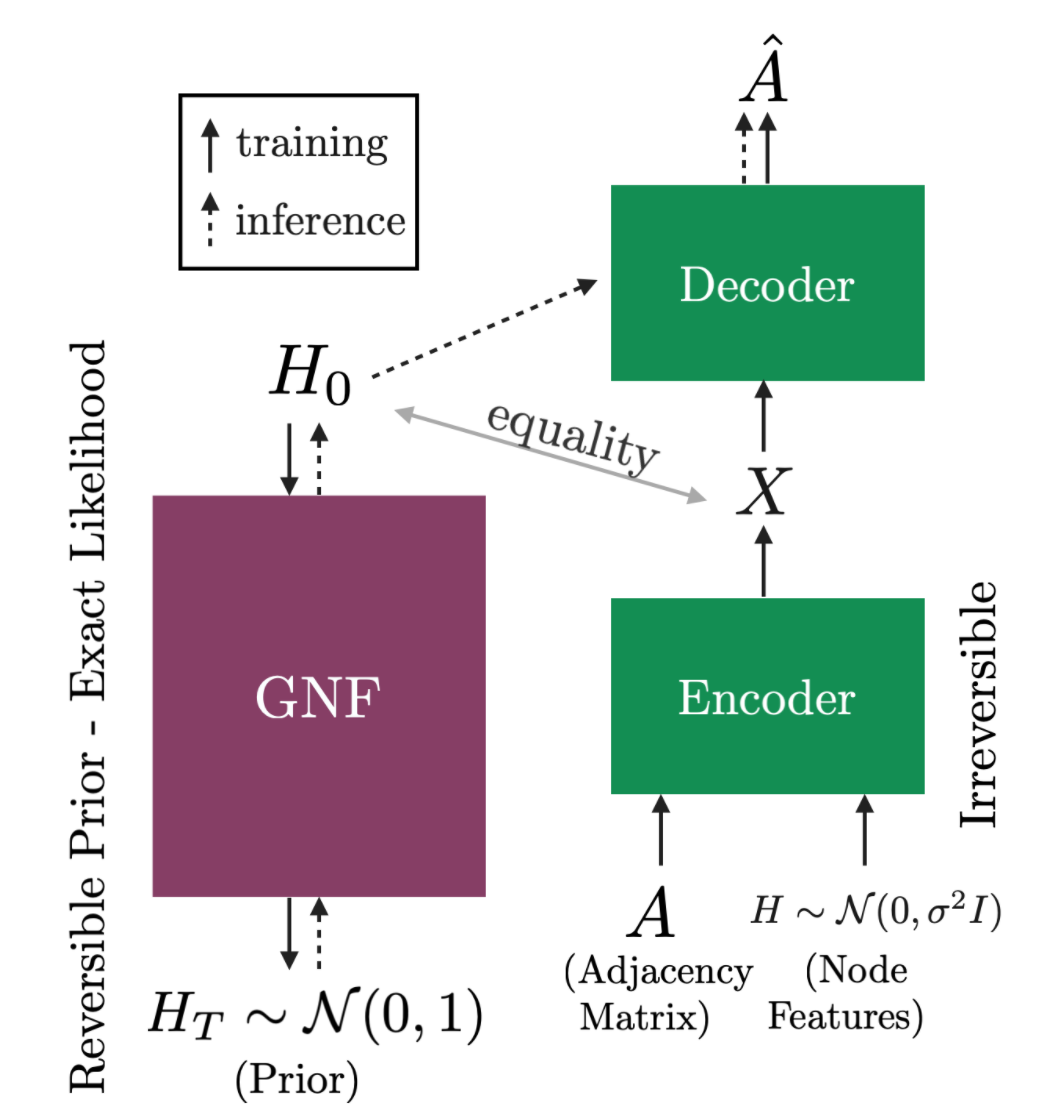
\includegraphics[width=2.0in]{./images/full_arch_gnf.png}
\caption{\label{fig:figure name}figure name}
\end{figure}
\begin{itemize}
\item Graphite isotropic gaussian for VAE + iterative refinement for decoding
\end{itemize}
\subsection{Three most popular according to O'Bray 2021:}
\label{sec:org2822432}
\begin{itemize}
\item GraphRNN, GRAN, Graph Score Matching.
\end{itemize}

\section{Objective:}
\label{sec:orgbea99e2}
\subsection{Generative graph dist close to the input graph dist}
\label{sec:orge5030dd}
\subsection{(pseudo)-metric to assess dissimilarity between G (generated graphs) and G* (input graphs)}
\label{sec:org646e1e7}

\section{Criteria for good metrics:}
\label{sec:org5e3d246}
\begin{enumerate}
\item Robust to noise
\item Expressive, if they don't arise from the same dist, then metric should detect this.
\item Computationally efficient.
\end{enumerate}

\section{Problems with Frechet Inception Distance}
\label{sec:org5f06944}
\begin{itemize}
\item Used only for images.
\item Perceived differences are not possible for graphs.
\item How about LPIPS?
\end{itemize}

\section{Why comparing graphs is hard:}
\label{sec:orgd5aecb8}
\begin{itemize}
\item Metrics need to deal with spatial invariances such as cycles.
\item Graph edit distance is NP-hard (Zeng 2009) and therefore does not satisfy efficiency criterion.
\end{itemize}

\section{MMD - current accepted method to evaluate generative GNNs}
\label{sec:orgeea2349}
\begin{itemize}
\item The MMD formula goes as follows:\begin{equation*}
\end{itemize}
\(\text{MMD}(X, Y) := {1\over n^2} \sum_{i,j=1}^{n}k(x_i, x_j) + {1\over m^2} \sum_{i,j=1}^{n}k(y_i, y_j) - {2\over nm} \sum_{i=1}^{n}\sum_{j=1}^{m}k(y_i, y_j)\)
\begin{itemize}
\item use it for hypothesis/two-sample testing.
\item In practice, we evaluate \(d_{MMD}(\mathcal{G},\mathcal{G*}) :=
  MMD(f(\mathcal{G}),f(\mathcal{G}*))\) for a distribution \(\mathcal{G}\). Given
multiple distributions \(G_1, G_2, \hdots\), the values of \(d_{MMD}\) can be used
to rank models, where smaller values are assumed to indicate a larger
agreement with the original distribution \(\mathcal{G}*\).
\item Commonly used kernels: first Wasserstein distance, total variation distance,
radial basis function.
\item Commonly used descriptor functions: degree distribution histogram, clustering
coefficient, laplacian spectrum histogram.
\end{itemize}
\subsection{Pitfalls of descriptors}
\label{sec:org29e11db}
\begin{itemize}
\item Degree distributions are ok seemingly
\item Custering does not distinguish fully connected vs disconnected cliques
\item Spectral methods are not clearly expressive. Does not seem to be for certain classes of graphs.
\end{itemize}

\section{MMD pitfalls}
\label{sec:orge0585d9}
\subsection{Parameters and descriptors are set a priori in the best case}
\label{sec:org8aad64c}
\subsection{Model performance is highly dependent on parameters and descriptor functions.}
\label{sec:orge48080c}



\section{Computer Vision}
\label{sec:org24bdf33}
\subsection{Image-to-Image Translation}
\label{sec:org900a111}
\subsubsection{CycleGAN: Unpaired Image-to-Image Translation using}
\label{sec:org8a0a19b}
Cycle-Consistent Adversarial Networks citep:zhu2017CycleGAN.



This is one of my favorite papers. The authors extending some
of the classic work done in Pix2Pix citep:isola2017pix2pix to
\emph{unpaired} sets of images. At the core of the CycleGAN
procedure are two Generative Adversarial Networks that learn
to map images between two domains. The key addition that makes
this process work is an additional loss term, which enforces
that images passed through both generators should be as close
as possible to the input image. This has practical motivation:
if we translate one way and then translate back, we should
expect the input to be unchanged. The results are impressive
and eye catching. This work inspired a paper of mine:
GeneSIS-RT.

\section*{References}
\label{sec:orgc73ae68}
\printbibliography[heading=none]
\end{document}